
%***********************************************************************

% This is a template to be used for the preparation of
% papers submitted to the 34th International Workshop on
% Statistical Modelling, to be held in Trieste, Italy,
% July 18-22, 2022.

% Please follow the following general guidelines:
%
% (1) Do not specify any definitions, commands or style parameters.
%     Upon submission, your file will be checked for presence of
%     \newcommand or \def statements and if found, error message will be reported
%     by the submission form.
%
% (2) Follow the template below very tightly.
%
% (3) Include .pdf figures using the \includegraphics
%      command, an example of which are given below.
%
% (4) Use file names which begin with the surname of the first author.
%
% (5) When creating labels for cross-references, please start always
%     by surname of the first author, e.g., \label{smith:likelihood}
%
% (6) The template below contains some example materials
%      to guide you through the preparation of your paper.  However,
%      remove all the redundant material from your final document
%      before submitting.

% The guidelines above are needed in order to be able to combine all
% the papers into a single proceedings book of acceptable quality.
% Please follow the guidelines as strictly as possible. Deviations may
% result in papers being either refused by the registration form
% or sent back to the authors with the request to change
% their documents according to the guidelines.

% Special characters:
% Please do not use special characters (e.g., accents).
% Use TeX composition instead, such as \~n, \'a, \`e, \v{s}, \r{u} etc.

% Changes as of IWSM 2013:
%  * \usepackage{booktabs} added which allows \toprule et al. in the tabular environment
%    (\hline\hline is not longer used)
%  * '^\T' added in iwsm.sty to denote transposed vectors and matrices within math (see example below)
%  * \usepackage{amsmath, amssymb} introduced since IWSM 2012 is allowed (allowing usage of boldsymbols
%    and other handy constructions (align, pmatrix etc.) within math)
%  * \usepackage{psfrag} introduced since IWSM 2012 is NOT allowed
%
%

%***********************************************************************
% PLEASE LEAVE THIS PART UNCHANGED
%***********************************************************************

\documentclass[twoside]{report}
\usepackage{iwsm}
\usepackage{graphicx}
\usepackage{amsmath, amssymb}
\usepackage{booktabs}

% Please do not specify any new definitions, any new commands,
% and do not specify any style parameters.
% The preamble of the document should be left unchanged.

\begin{document}

%***********************************************************************
% PLEASE INSERT YOUR CONTENT FROM HERE
%***********************************************************************

% Title and running title to be used as left header:
\title{Probabilistic Precipitation Forecasts: Model comparison and Graphical Assessment}
\titlerunning{Probabilistic Precipitation Forecast Assessment}

% Authors and running list of authors to be used as right header:
\author{Reto Stauffer\inst{1}\inst{2}, Moritz N. Lang\inst{1}, Achim Zeileis\inst{1}}
\authorrunning{Surname 1 et al.}    %% use \authorrunning{Surname 1} if only 1 author
                                    %% use \authorrunning{Surname 1 and Surname2} if two authors
                                    %% use \authorrunning{Surname 1 et al.} if more than two authors

% Institutes of all authors
% Include city and country of each institute, do not include the full address.
\institute{Department of Statistics, Universit\"at Innsbruck, Austria
\and Digital Science Center, Universit\"at Innsbruck, Austria}

% E-mail of presenting author for correspondence
\email{Reto.Stauffer@uibk.ac.at}

% Brief abstract of the paper:
\abstract{
    The demand of accurate and reliable probabilistic precipitation forecasts
    has seen an increase over the past decades, especially under the current
    changing climate which shows an increase in frequency and intensity of
    severe precipitation events.

    Probabilistic weather forecasts are typically generated by physically
    based numerical ensemble models providing multiple forecasts with slightly
    different conditions to depict the forecast uncertainty for a specific situation.
    Due to the nature of the data and the necessary simplifications these forecasts
    are not perfect and often show too little uncertainty, especially when compared
    to sprcific locations.

    Statistical post-processing is thus commonly used to increase the accuracy
    and reliability. Distributional regression models have shown to be compatible
    with other methods proposed over the past decade and allow to not only correct
    the expectation, but to simultanously adjust the uncertainty.
    Proper scoring rules, e.g., CPRS or log-scores, are often used to find the
    best performing model alongside with graphical assessment methods. The latter
    can be particularely useful to identify possible misspecifications in the
    model assumption and will be the focus of this contribution.
}

% Keywords (at most 5):
\keywords{Distributional regression; precipitation forecasts; graphical model assessment}

% Produce the title:
\maketitle

%***********************************************************************

% Sections and subsections (do not use lower levels):

\section{Introduction/Background}

Forecasting precipitation has always been one of the essential quantities in
weather forecasting not only for the public, but for many socio-economic areas
like agriculture, power production, but also decison makers with respect risk
assessments. 
The demand of accurate predictions of the expected amount of precipitation has
increased over the past decade where severe precipitation events have increased
in intensity and frequency.

Weather forecasts are typically generated by physically based numerical weather
prediction models. To account for uncertainty, multiple forecasts are created
with slightly modified conditions which build an ensemble (Gneiting et\,al.
2005). This allows to not only retrieve the expected amount of precipitation
but information about the uncertainty of a specific forecast.
To unleash the full potential of these ensemble forecasts, statistical
post-procesing is often used to correct model biases and insufficiencies in
forecast uncertainty. This is especially important when comparing the raw
ensemble forecasts to different spatial scales, e.g., to specific locations.

Probabilistic statistical methods allow to simultanously adjust the
expectation 
...
[Ab ins naechste Meeting]
Over the recent years many probabilistic statistical post-processing methods
have been proposed. .....
allows to imrpove the accuracy and reliability
of these forecasts by comparing historical ensemble forecast and observed
amounts to correct for possible errors.

In the recent past many different
statistical models have been proposed using different distributional assumptions
and learners. For evaluation, proper scoring rules are often used which not
only evaluate the expectation but the full probabilistic distribution of
the forecasts. To identify possible misspecifications in the model
assumption, graphical assessment methods are particularely advantageous
and will be presented in this article.

\section{Data}

Toy data set consisting of X days of accumulated 3-day precipitation
forecasts for station Innsbruck and corresponding observations.

\section{Methodology}

\subsection{Statistical models}

\subsection{Model assessment}

$$
y_i \sim \mathcal{D}(\theta_i | X_i)
$$

Rootogram (Marginal scale):

$$
\text{obs}_j = \sum_{i=1}^n \omega_i I(y_i \in (b_j, b_{j+1}))
$$

$$
\text{exp}_j = \sum_{i=1}^n \omega_i \big[ F(b_{j+1} | \hat{\theta}_i) - F(b_{j} | \hat{\theta}_i) \big],
$$

PIT residuals; CDF evaluated at observation $y_i$ given the
estimated parameters $\hat{\theta}_i$.

$$
u_i = F(y_i | \hat{\theta}_i)
$$


QQ-residuals

$$
\hat{r}_i = \Phi^{-1}\big(F(y_i | \hat{\theta}_i)\big) = \Phi^{-1}(u_i)
$$

for the theoretical quantiles ($z_i$) one typically draws $N$ equidistant
quantiles from the Normal distribution ($\frac{1}{N+1}, ..., \frac{N}{N+1}$),
plotting all pairs $\big((z_{(1)},\hat{r}_{(1)}), ..., (z_{(N)},\hat{r}_{(N)})\big)$

Wormplots: basically the same but detrended

$\big((z_{(1)},\hat{r}_{(1)} - z_{(1)}), ..., (z_{(N)},\hat{r}_{(N)} - z_{(N)})\big)$

\section{Model comparison}

Show plots here, refer to the equations above.

\begin{figure}[!ht]\centering
    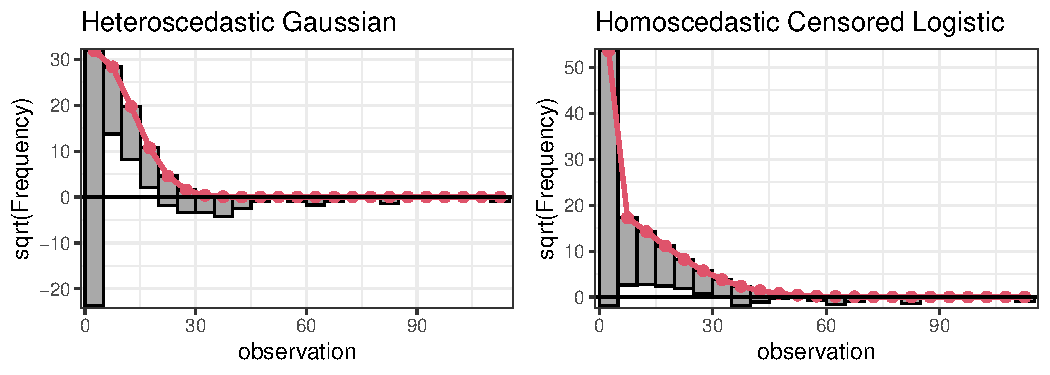
\includegraphics[width=\textwidth]{Stauffer-rootograms}
    \caption{\label{stauffer:fig1} Caption text \textbf{BELOW} the figure.}
\end{figure}

\begin{figure}[!ht]\centering
    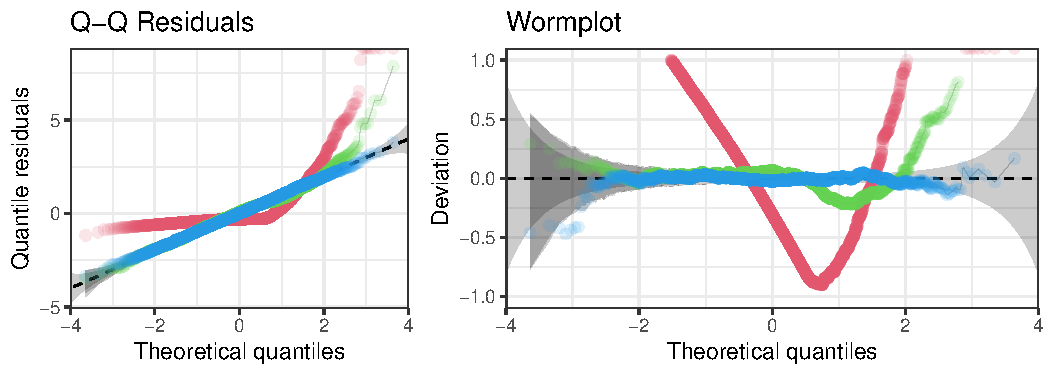
\includegraphics[width=\textwidth]{Stauffer-qqresiduals}
    \caption{\label{stauffer:fig2} Caption text \textbf{BELOW} the figure.}
\end{figure}


%***********************************************************************

% Acknowledgments, if needed:
\acknowledgments{Special Thanks to ... }

%***********************************************************************

% References should be placed in the text in author (year) form.
% The list of references should be placed below IN ALPHABETICAL ORDER.
% (Please follow the format of the examples very tightly).




\references
\begin{description}
% Reliability diagram
\item [Bröcker, J., and Smith, L.A.] (2007).
    Increasing the Reliability of Reliability Diagrams.
    {\it Weather and Forecasting},
    {\bf 22}(3), 651\,--\,61.
% Ensemble forecasting
\item[Gneiting, T, and Raftery, A.E.] (2005).
    Weather Forecasting with Ensemble Methods.
    {\it Science},
    {\bf 310}(5746), 248\,--\,249.
% Proper scoring rules (CRPS)
\item[Gneiting, T, and Raftery, A.E.] (2007).
    Strictly Proper Scoring Rules, Prediction, and Estimation.
    {\it ournal of the American Statistical Association},
    {\bf 102}(477), 359\,--\,78.
% Maximize sharpness subject to calibration
\item[Gneiting, T., Balabdaoui, F., and Raftery, A.E.] (2007).
    Probabilistic Forecasts, Calibration and Sharpness.
    {\it Journal of the Royal Statistical Society: Series B (Methodological)},
    {\bf 69}(2), 243\,--\,68.
% Rootograms (marginal calibration)
\item [Kleiber, C., and Zeileis A.] (2016).
    Visualizing Count Data Regressions Using Rootograms.
    {\it The American Statistician},
    {\bf 70}(3): 296\,--\,303.
% PIT residuals (specifically)
\item [Warton, D.I., Thibaut, L., and Wang, Y.A.] (2017).
    The Pit-Trap---{A} ``Model-Free'' Bootstrap Procedure for Inference About
    Regression Models with Discrete, Multivariate Responses.
    {\it PLOS ONE},
    {\bf 12}(7), 1\,--\,18.
% Reliability diagram
\item [Wilks, D.] (2011).
    {\it Statistical Methods in the Atmospheric Sciences 3rd ed}.
    Academic Press.
\end{description}

\end{document}
